\documentclass[addpoints,spanish, 12pt,a4paper]{exam}
%\documentclass[answers, spanish, 12pt,a4paper]{exam}
\printanswers
\pointpoints{punto}{puntos}
\hpword{Puntos:}
\vpword{Puntos:}
\htword{Total}
\vtword{Total}
\hsword{Resultado:}
\hqword{Ejercicio:}
\vqword{Ejercicio:}

\usepackage[utf8]{inputenc}
\usepackage[spanish]{babel}
\usepackage{eurosym}
%\usepackage[spanish,es-lcroman, es-tabla, es-noshorthands]{babel}


\usepackage[margin=1in]{geometry}
\usepackage{amsmath,amssymb}
\usepackage{multicol}
\usepackage{yhmath}

\pointsinrightmargin % Para poner las puntuaciones a la derecha. Se puede cambiar. Si se comenta, sale a la izquierda.
\extrawidth{-2.4cm} %Un poquito más de margen por si ponemos textos largos.
\marginpointname{ \emph{\points}}

\usepackage{graphicx}

\graphicspath{{../../img/}} 

\newcommand{\class}{1º Bachillerato CCSS}
\newcommand{\examdate}{\today}
\newcommand{\examnum}{Parcial 1 - Pendientes}
\newcommand{\tipo}{A}


\newcommand{\timelimit}{105 minutos}

\renewcommand{\solutiontitle}{\noindent\textbf{Solución:}\enspace}


\pagestyle{head}
\firstpageheader{
\includegraphics[width=0.2\columnwidth]{header_left}}{\textbf{Departamento de Matemáticas\linebreak \class}\linebreak \examnum}{
\includegraphics[width=0.1\columnwidth]{header_right}}
\runningheader{\class}{\examnum}{Página \thepage\ of \numpages}
\runningheadrule


\usepackage{pgf,tikz,pgfplots}
\pgfplotsset{compat=1.15}
\usepackage{mathrsfs}
\usetikzlibrary{arrows}


\begin{document}

\noindent
\begin{tabular*}{\textwidth}{l @{\extracolsep{\fill}} r @{\extracolsep{6pt}} }
\textbf{Nombre:} \makebox[3.5in]{\hrulefill} & \textbf{Fecha:}\makebox[1in]{\hrulefill} \\
 & \\
\textbf{Tiempo: \timelimit} & Tipo: \tipo 
\end{tabular*}
\rule[2ex]{\textwidth}{2pt}
Esta prueba tiene \numquestions\ ejercicios. La puntuación máxima es de \numpoints. 
La nota final de la prueba será la parte proporcional de la puntuación obtenida sobre la puntuación máxima. 

\begin{center}


\addpoints
 %\gradetable[h][questions]
	\pointtable[h][questions]
\end{center}

\noindent
\rule[2ex]{\textwidth}{2pt}

\begin{questions}

\question[8] Resolver por el método de Gauss los siguientes sistemas:
		$$\left\{ {\begin{array}{*{20}{c}}
  {x{\text{ }} + {\text{ 2y     }} = {\text{  1}}} \\ 
  {{\text{ - 2x }} + {\text{ 3y }} + {\text{ z }} = {\text{  - 1}}} \\ 
  {{\text{3x  -  y  }} - {\text{z }} = {\text{ 2}}} 
\end{array} } \right.$$
\begin{solution}
% A=Matrix(3,4,[1,2,0,1,-2,3,1,-1,3,-1,-1,2])
$A^*=\left(\begin{matrix}1 & 2 & 0 & 1\\-2 & 3 & 1 & -1\\3 & -1 & -1 & 2\end{matrix}\right)\sim\left(\begin{matrix}1 & 2 & 0 & 1\\0 & 7 & 1 & 1\\0 & 0 & 0 & 0\end{matrix}\right)\to x=\frac{2 \lambda}{7} + \frac{5}{7}, y=\frac{1}{7} - \frac{\lambda}{7}, z=\lambda$ \\

\end{solution}
\question[10] Resuelve las siguientes inecuaciones:
\begin{parts}
    \part $\dfrac{{{\text{3}}\cdot{\text{(x - 1)}}}}{{\text{2}}}{\text{  -  4x }} < {\text{ 1  -  }}\left( {{\text{x }} + {\text{ }}\frac{{\text{1}}}{{\text{2}}}} \right)$
    \begin{solution}
        $-3x < 4 \to (-\frac{4}{3}, \ \infty)$
    \end{solution}
    \part $\dfrac{{{x^2} - 25}}{{{x^2} - 7x + 10}}{\text{ }} \leqslant {\text{ 0 }}$
    \begin{solution}
        $ \dfrac{(x+5)(x-5)}{(x-5)(x-2)}\leqslant0  \to [-5, \ 2)$
    \end{solution}
\end{parts}

\question[8] Resuelve el siguiente sistema de inecuaciones:
\[\left\{ {\begin{array}{*{20}{c}}
  {{\text{x }} + {\text{ y }} \leqslant {\text{ 3}}} \\ 
  {{\text{2x }} + {\text{ y }} \geqslant {\text{ 8}}} \\ 
  {{\text{x }} \geqslant {\text{ 0}}} \\ 
  {{\text{y }} \geqslant {\text{ 0}}} 
\end{array}} \right.\]
\begin{solution}
    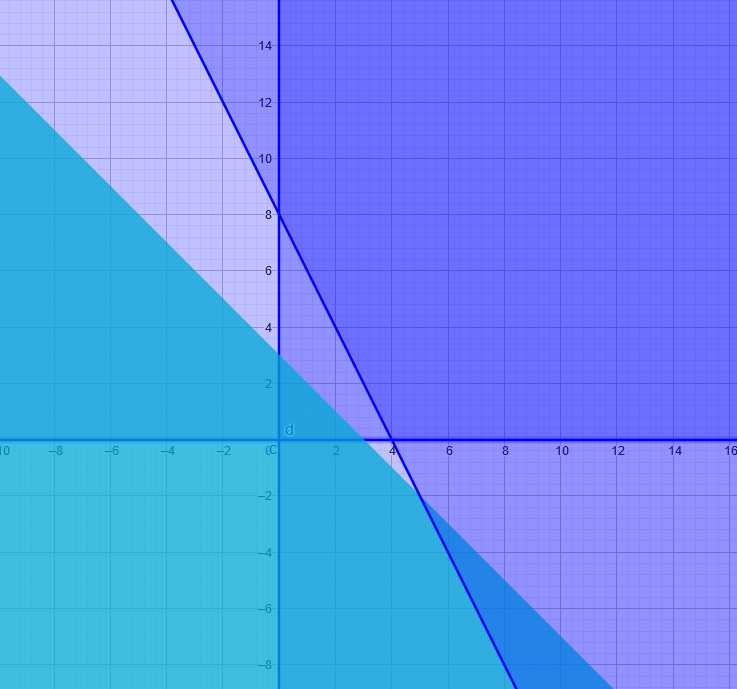
\includegraphics[width=10cm]{pendientes_1_bach/1_sociales/prog_lin.png} \\
    Como no tiene intersección, el sistema no tiene solución
\end{solution}



\question[10] Una empresa cinematográfica dispone de tres salas A, B y C. Los precios de entrada a cada una de estas salas son 1, 2 y 3\euro \ respectivamente. Un día la recaudación conjunta de las tres salas fue de 425\euro \ y el número total de espectadores que acudieron fue de 200. Si los espectadores de la sala A, hubiesen asistido a la sala B y los de la sala B a la sala A, se obtendría una recaudación de 400\euro. Calcula el número de espectadores que acudió a cada sala.
\begin{solution}
    $\left\{ \begin{matrix}x + 2 y + 3 z = 425 \\ x + y + z = 200 \\ 2 x + y + 3 z = 400 \\ \end{matrix}\right.$ \\
    $A^*=\left(\begin{matrix}1 & 2 & 3 & 425\\1 & 1 & 1 & 200\\2 & 1 & 3 & 400\end{matrix}\right)\sim\left(\begin{matrix}1 & 2 & 3 & 425\\0 & -1 & -2 & -225\\0 & 0 & 3 & 225\end{matrix}\right)\to x=50, y=75, z=75$
\end{solution}

\question[20] Resuelve las siguientes ecuaciones:
\begin{parts}
    \part $\sqrt {x - 3} {\text{ }} + {\text{ }}\sqrt {{\text{3x - 5}}} {\text{ }} = {\text{ 6}}$
    \begin{solution}
        $x^{2} - 74 x + 469=0 \to [7,67] \to x=7$
    \end{solution}
    \part $2 \log (x+3) - \log (x-6) = 2$
    \begin{solution}
        $\dfrac{(x+3)^2}{(x-6)}=100 \to x= 7,   x=87$
    \end{solution}
    \part $3^{x-1} + 3^{x+2} = 84$
    \begin{solution}
        $3^x(\frac{1}{3}+9)=84 \to 3^x=\frac{84\cdot 3}{28} \to 3^x=9 \to x=2$
    \end{solution}
    \part $x^5 - 3x^4 - 8x^3 + 12x^2 + 16x = 0$
    \begin{solution}
        $x \left(x - 4\right) \left(x - 2\right) \left(x + 1\right) \left(x + 2\right)=0 \to x=0, x=4, x=2, x=-1, x=-2$
    \end{solution}
\end{parts}
\question[9] Opera, simplifica y racionaliza en todos los casos en que se presente:
\begin{parts}
    \part $\frac{3}{{4\sqrt 2 }}$
    \begin{solution}
        $\frac{3 \sqrt{2}}{8}$
    \end{solution}
    \part $\frac{{\sqrt 6 \, - \,\sqrt 2 }}{{\sqrt {12}  - 2}}$	
    \begin{solution}
        $\dfrac{(\sqrt{6}-\sqrt{2})(2\sqrt{3}+2)}{4\cdot 3 - 4}=\dfrac{\sqrt{2}(\sqrt{3}-1)\cdot 2(\sqrt{3}+1)}{8}=\frac{4\sqrt{2}}{8}=\frac{\sqrt{2}}{2}$
    \end{solution}
    \part $\sqrt[5]{{{2^2}\sqrt[4]{{8\sqrt[3]{2}}}}}.\sqrt[{30}]{{{2^{43}}}}$
    \begin{solution}
        $\sqrt[60]{2^{34}}\cdot \sqrt[60]{2^{86}}=\sqrt[60]{2^{120}}=2^2=4$
    \end{solution}
\end{parts}

\question La cotización en bolsa (en miles de \euro) de los dos valores Minerocat (X) y Construcat (Y) a lo largo de 6 días de sesión son los siguientes:
\begin{center}
\begin{tabular}{|c|c|c|c|c|c|c|}
    \hline
    X= Minerocat & 8 & 7 & 6 & 5 & 7 & 8 \\
    \hline
    Y= Construcat & 6 & 5 & 4.5 & 4 & 4.5 & 5  \\
    \hline
\end{tabular}
   
\end{center}

\begin{parts}
    \part[9] Calcula el coeficiente de correlación de Pearson. Da una interpretación del mismo en términos del enunciado del problema
    \part[6] La cotización en bolsa de Minerocat alcanza el valor 9 un cierto día, ¿qué cotización en bolsa cabe esperar que alcance el valor Construcat?. Es correcta la predicción
\end{parts}
\begin{solution}
\begin{tabular}{lrrrrr}
\hline
        &        a &        b &   $a\cdot b$ &    $a^2$ &   $b^2$ \\
\hline
 0      &  8       &  6       &      48      &  64      &   36    \\
 1      &  7       &  5       &      35      &  49      &   25    \\
 2      &  6       &  4.5     &      27      &  36      &   20.25 \\
 3      &  5       &  4       &      20      &  25      &   16    \\
 4      &  7       &  4.5     &      31.5    &  49      &   20.25 \\
 5      &  8       &  5       &      40      &  64      &   25    \\
 Sumas  & 41       & 29       &     201.5    & 287      &  142.5  \\
 Medias &  6.83333 &  4.83333 &      33.5833 &  47.8333 &   23.75 \\
\hline
\end{tabular}
\\ \\ Las medias son: \\$\overline{a}=\frac{\Sigma{a_i}}{N}=\frac{41.0}{6}=6.83333333333333$. $\overline{b}=\frac{\Sigma{b_i}}{N}=\frac{29.0}{6}=4.83333333333333$.  El centro de gravedad es: $(6.83333333333333,4.83333333333333)$ \\ \\ Varianzas y covarianzas: \\ $\sigma_a=\sqrt{\frac{\sum{a_i^2}}{N}-\overline{a}^2}=\sqrt{\frac{287.0}{6}-6.83333333333333^2}=1.06718737290548$.\\ $\sigma_b=\sqrt{\frac{\sum{b_i^2}}{N}-\overline{b}^2}=\sqrt{\frac{142.5}{6}-4.83333333333333^2}=0.623609564462327$.\\ $\sigma_{ab}=\frac{\sum{a_i \cdot b_i}}{N}-\overline{a}\cdot \overline{b}=\frac{201.5}{6}-6.83333333333333\cdot 4.83333333333333=0.555555555555564$. \\ \\ Correlación: \\ $r=\dfrac{\sigma_{ab}}{\sigma_a \cdot \sigma_b}=\frac{0.555555555555564}{1.06718737290548\cdot 0.623609564462327}=0.83478387112969$. \\ \\ Recta de regresión: \\ La pendiente es: 0.48780487804878, la ordenada en el origen: 1.5, El coeficiente de correlación:0.834783871129682 y la recta de regresión: $y = 0.48780487804878 x + 1.5$
\\

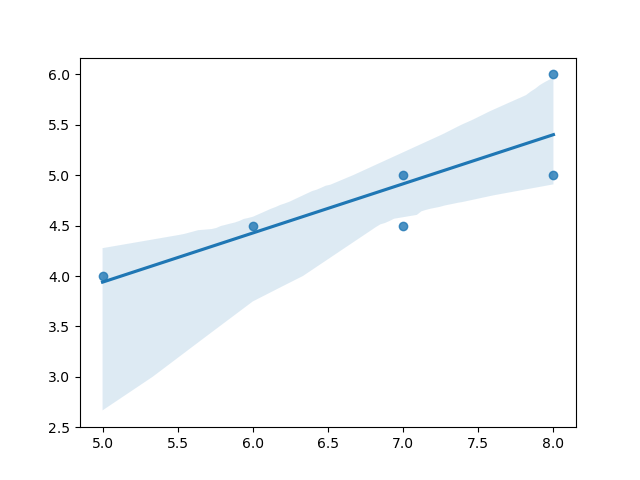
\includegraphics[width=8cm]{pendientes_1_bach/1_sociales/regresion1.png} 
\\

Estimación para $x=9$:
$y=5.89024390243902$

\end{solution}
\end{questions}

\end{document}
\grid
